\documentclass[11pt]{article}
\usepackage[utf8]{luainputenc}
\usepackage[T1]{fontenc}
\usepackage{amsmath,amsfonts,amssymb} 
\usepackage{mathtools, thmtools}
\usepackage[margin=1in]{geometry}
\usepackage[onehalfspacing]{setspace}
\usepackage{xcolor, graphicx}
\usepackage{caption}
\usepackage{subcaption}
\usepackage[colorlinks, citecolor=blue]{hyperref}
\usepackage[noabbrev, capitalize, nameinlink]{cleveref}
\usepackage{csquotes}

\newtheorem{Theorem}{Theorem}[section]
\newtheorem{Corollary}[Theorem]{Corollary}
\newtheorem{Proposition}[Theorem]{Proposition}
\newtheorem{Lemma}{Lemma}[section]
\newtheorem{Assumption}{Assumption}[section]

\newcommand*{\R}{\mathbb{R}}
\newcommand*{\E}{\mathbb{E}}
\newcommand*{\N}{N}
\newcommand*{\Var}{\mathbb{V}ar}
\newcommand*{\pto}{\stackrel{p}{\to}}
\newcommand*{\dto}{\stackrel{d}{\to}}
\DeclarePairedDelimiter\abs{\lvert}{\rvert}
\DeclarePairedDelimiter\norm{\lVert}{\rVert}
\newcommand{\mvert}[1][\middle]{\ensuremath{\,#1\vert\,}}
\renewcommand{\arraystretch}{1.4}

\usepackage[backend=biber, autopunct=true, authordate, hyperref=true]{biblatex-chicago} 
\addbibresource{riskpriceinference.bib}
\graphicspath{{figures/}}

\author{Xu Cheng, Eric Renault, \& Paul Sangrey}
\title{Inference for the Price of Risk Under Weak Identification}
\date{\today}

\begin{document}

\maketitle

Two key questions at the very heart of fiance are what are the risks investors face and what are the prices of
those risks.
Two leading risks are equity risk and volatility risk.
Although the literature has shown that volatility risk clearly matters, constructing beliefs concerning the price
of volatility risk from the data has proven quite difficult.
What we want is a good estimator for this parameter and a strategy for credible inference regarding it.  

We take the model from \textcite{khrapov2016affine} and use it to estimate the relevant
parameters, which we derive below. 
We use spectral GMM, which forms moment conditions from the characteristic function.
Out data we use are the bivariate series $\begin{pmatrix} r_{t+1}, \sigma^2_{t+1} \end{pmatrix}$.
$r_{t+1}$ is the daily return on some asset, and we use its associated realized volatility for $\sigma^2_{t+1}$.

Moving forward, we sketch the model developed in \textcite{khrapov2016affine} and derive the associated moment
conditions.
We then provide a series of sufficient conditions for valid inference. 
We have a pricing kernel $M_{t, t+1}(\theta)$ which allows us to characterize the price $P_t$ at time $t$ of any
payoff at time $t+1$ of a function $f$ and information set $I_t$, $f\left(r_{t+1}, \sigma^2(t+1) \mvert
I_t\right)$. 
We use $*$'s to denote the risk neutral measure.

\begin{equation}
    P_t  = \E\left[M_{t,t+1}(\theta) f\left(r_{t+1}, \sigma^2(t+1) \mvert  I_t\right) \mvert I_t \right] =
    \E^{*}\left[H(r_{t+1}, \sigma^2(t+1),  I_t) \mvert I_t \right] 
\end{equation}


To make the problem tractable, we assume that the problem is Markov and that there is no Granger causality from
return to volatility. 
This implies the conditional probability distribution of $\sigma^2_{t+1} \vert I_t$ equals the conditional
probability distribution of $\sigma^2_{t+1} \vert \sigma^2_t$.
Consequently, we can write down our model in the risk-neutral measure using some functions, $a^{*}(u), b^{*}(u)$,
and $\alpha^{*}(v), \beta^{*}(v), \& \gamma^{*}(v)$, as the following two equations in terms of the Laplace
transforms of the probability distributions.

\begin{align}
    \E^{*}\left[\exp\left(-x \cdot \sigma^2_{t+1}\right) \mvert \sigma^2_t\right] &= \exp\left(-a^{*}(x)
    \sigma_t^2 - b^{*}(x)\right) \\
    \E^{*}\left[\exp\left(-x \cdot r_{t+1} \right)\mvert \sigma^2_t \sigma^2_{t+1}\right] &=
    \exp\left(-\alpha^{*}(x) \sigma^2_{t+1} - \beta^{*}(x) \sigma^2_t - \gamma^{*}(x)\right)
\end{align}


\section{The Model}


We assume that the volatility follows an autoregressive gamma process---ARG(1), and so its physical measure
dynamics are governed by following equations.

\begin{gather}
    a(x) = \frac{\rho x}{1 + c x}  \\
    b(x) = \delta \log \left(1 + c x\right) \\
    \rho \in [0, 1), c > 0, \delta > 0 
\end{gather}

The persistence is governed by $\rho$, and the mean by $\delta$, and $c$ is a scaling factor for the volatility as
can be seen in the formula for $\sigma^2_{t+1}$'s conditional mean.

\begin{equation}
    \E\left[\sigma^2_{t+1} \mvert \sigma^2_t\right] = c \delta + \rho \sigma^2_t
\end{equation}

Assuming the measure change preserves the general structure between the risk-neutral and physical measures implies
\cref{eqn:cond_characterisitc_func}.
We also assume that $\left[ \frac{\psi}{\phi} \right]^2 \approx \frac{\E \left[\sigma^2_{t+1} \mvert
I_t\right]}{\Var\left[r_{t+1} \mvert I_t\right]}$, which enables our approximation of $\sigma^2_{t+1}$ by the
realized volatility.

\begin{equation}
    \label{eqn:cond_characterisitc_func}
    \E\left[\exp\left(- x \cdot r_{t+1}\right) \mvert \sigma_t^2, \sigma^2_{t+1}\right] = \exp\left(- a(x)
    \alpha^2_{t+1} - \beta(x) \sigma^2_t - \gamma(x) \right) 
\end{equation}

To estimate this equation, we need to know all of the relevant functions.
The parametric structure of the problem and some algebra implies the following.

\begin{align}
    a(x) &= \frac{\rho x}{1 + c x} \\
    b(x) &= \delta \log \left(1 + c x\right) \\
    \alpha(x) &= \psi x - \frac{1}{2} x^2 (1 - \phi^2) \\
    \label{eqn:beta_defn}
    \beta(x)  &= x \alpha^{*}\left(- \frac{\phi}{\sqrt{c [1 + \rho]}} \right) \\
    \label{eqn:gamma_defn}
    \gamma(x) &= x b^{*}\left(- \frac{\phi}{\sqrt{c [1 + \rho]}}\right) 
\end{align}

In last two of the above equations we have the risk-neutral $\alpha^{*}(x)$ and $\beta^{*}(x)$ functions which we
have not defined.
To solve for them we drive the implied stochastic discount factor and make the appropriate measure change.
We parameterize the SDF in terms of price of volatility risk---$\theta_1$---and the price of equity risk---$\theta_2$.
The SDF satisfies the following equation for some functions $m_0(\cdot)$ and $m_1(\cdot)$.

\begin{gather}
    M_{t,t+1}(\theta) = \exp(-r_{f,t}) \exp\left(m_{0}(\theta) + m_1(\theta) \sigma_t^2 - \theta_1 \sigma^2_{t+1}
    - \theta_2 r_{t+1}\right) \\
    \intertext{Then by the law of iterated expectations and some algebra.}
    \E \left[\exp\left(m_{0}(\theta) + m_1(\theta) \sigma_t^2 - \theta_1 \sigma^2_{t+1} - \theta_2 r_{t+1}\right)
    \exp\left(- \alpha(\theta_2) \sigma^2_{t+1} - \beta (\theta_2) \sigma^2_{t+1} - \gamma(\theta_2)\right) \mvert
    I_t \right] = 1
\end{gather}

This implies the two unspecified functions are as follows.

\begin{align}
    m_{0}(\theta) &= \gamma(\theta_2) + b\left(\alpha\left(\theta_2\right) + \theta_1\right) \\
    m_{1}(\theta) &= \beta(\theta_2) + a\left(\alpha(\theta_2) + \theta_1\right) 
    \intertext{Now we can solve for $\alpha^{*}(x)$ and $\beta^{*}(x)$.}
    a^{*}(x) &= a\left(x + \theta_1 + \alpha(\theta_2)\right) - a\left(\theta_1 + \alpha(\theta_2)\right) \\
    b^{*}(x) &= b\left(x + \theta_1 + \alpha(\theta_2)\right) - b\left(\theta_1 + \alpha(\theta_2)\right) 
\end{align}


We substitute them back into \cref{eqn:beta_defn} and \cref{eqn:gamma_defn} eliminating $\alpha^{*}(x)$ and
$\beta^{*}(x)$.

\begin{align}
    a(x) &= \frac{\rho x}{1 + c x} \\ \label{eqn:a(x)}
    b(x) &= \delta \log \left(1 + c x\right) \\ \label{eqn:b(x)}
    \alpha(x) &= x \left(\frac{\phi}{\sqrt{c (1 + \phi)}}  + (1 - \phi^2)\left(\theta_2 - \frac{1}{2}\right)\right)
    - \frac{1}{2} x^2 (1 - \phi^2) \\ \label{eqn:alpha(x)}
    \beta(x)  &= x \left(a\left(-\frac{\phi}{\sqrt{c(1+ \rho)}} + \theta_1 + \alpha(\theta_2)\right) -
        a\left(\theta_1 + \alpha(\theta_2)\right)\right) \\ \label{eqn:beta(x)}
    \gamma(x) &= x \left(b\left(-\frac{\phi}{\sqrt{c(1+\rho)}} + \theta_1 + \alpha(\theta_2)\right) -
        b\left(\theta_1 + \alpha(\theta_2)\right) \right)
\end{align}


The set of parameters we want to estimate is $\omega \coloneqq \lbrace c, \rho, \delta, \phi, \theta_1,
\theta_2\rbrace$.

\section{Spectral GMM}

We derive a set of moment conditions from the characteristic function above by evaluating it at a grid of points
in $[0,1] \times i [0,1]$. 
That is we can define a function $g_t(x, \omega)$

\begin{equation}
g_t(x, \omega) = Z_t \otimes \begin{bmatrix} \exp(- x \sigma^2_{t+1}) - \exp\left( - a(x) \sigma_t^2 - b(x)
    \right) \\ \exp\left(- x r_{t+1}\right) - \exp\left(- \alpha(x) \sigma^2_{t+1} - \beta(x) \sigma_2^t -
    \gamma(x)\right) \end{bmatrix}
\end{equation}

Where the instruments are given by \cref{eqn:instruments} for complex unit $i$. 

\begin{equation}
    \label{eqn:instruments}
    Z_t = \left[1, \exp\left(- i \sigma_t^2\right), \exp\left(-i \sigma^2_{t-2}\right)\right] 
\end{equation}

The implied unconditional moment restrictions are the following.  

\begin{equation}
    \E \begin{bmatrix}  \mathrm{Re} (g_t(x, \omega)) \\ \mathrm{Im} (g_t(x, \omega)) \end{bmatrix} = 0
\end{equation}


The optimal weighting matrix has its standard form as the precision matrix of the moments as long as we choose a
finite gird for $x$. 
If we use the entire continuum, handling the weights becomes more delicate. 
So we use only finitely many moments for now.
Since the exponential function is a strictly positive function, and we are considering a grid of $x$ values, a
sufficient condition for $\rho, \delta, \& c$ to be identified is for the relevant rows of $\nabla a(x)$ and
$\nabla b(x)$ to equal zero only at $\omega_0$ which are satisfied if $\rho, c, \delta > 0$.
Testing if if $\phi$ and $\theta_2$ are identified is somewhat trickier. 
Consider $\nabla \alpha(x)$. 
%TODO Reword this.
Since we are using a grid of $x$'s, and the gradient of $\alpha$ is a
nonlinear function of $x$, the first two rows of the \cref{eqn:alpha_gradient} imply $\phi$ is identified.

\begin{equation}
    \label{eqn:alpha_gradient}
    \nabla_{\phi, \theta_2, c}  \alpha(x) = \begin{bmatrix} \phi x^{2} + x \left(- 2 \phi \left(\theta_{2} -
    \frac{1}{2}\right) - \frac{\phi}{2 \sqrt{c} \left(\phi + 1\right)^{\frac{3}{2}}} + \frac{1}{\sqrt{c}
    \sqrt{\phi + 1}}\right) \\ x \left(- \phi^{2} + 1\right) \\ \frac{\phi x}{2 c^{\frac{3}{2}} \sqrt{\phi + 1}}
\end{bmatrix} 
\end{equation}

The top line of \cref{eqn:alpha_gradient} can be solved for $\theta_2$, which would create a local lack of
identification for $\theta_2$.
However, this point is ruled out by the other equations.
Consequently,  $\phi \in (-1,1], c > 0$, are sufficient to identify all of the parameters except for $\theta_1$,
the price of volatility risk.

If we plug in the estimated values of the parameters from \textcite{khrapov2016affine} into $\frac{\partial
\beta}{\partial \theta_1}$ and plot it as a function of $\phi$,  we get the following.
The scale is omitted because it is not meaningful. 
As can clearly be seen in \cref{fig:fig:gamma_diff_theta2}, there is a zero when $\phi = 0$.

\begin{figure}[htb]
    \centering
    \caption{Derivative of $\gamma(x)$ with respect to $\theta_2$}
    \label{fig:fig:gamma_diff_theta2}
    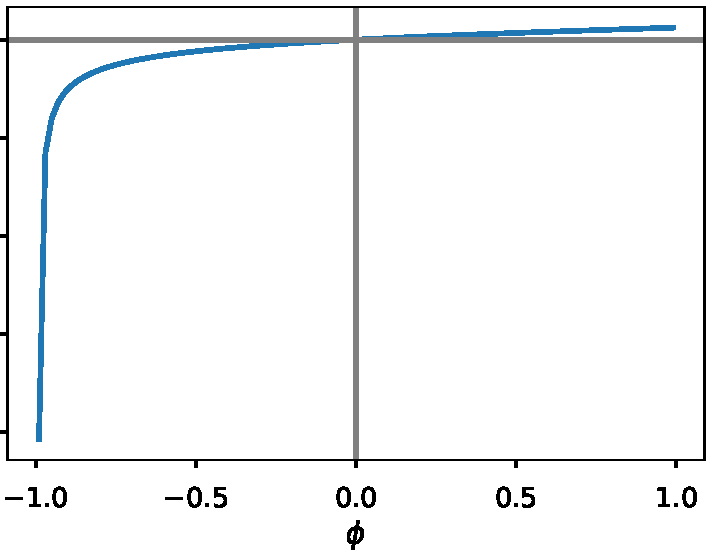
\includegraphics[width=.5\textwidth]{gamma_diff_theta2.pdf}
\end{figure}


For now, we will assume that $\phi \neq 0$, and hence the model is identified.
Hence, for any positive definite weight-matrix by \textcite[Lemma 2.3]{newey1994large} we are identified.
The data, $\sigma^2_{t+1}, r_{t+1}$, are ergodic and stationary.
Since the moment conditions are not redundant the optimal (GMM) weight matrix $W$ is positive definite. 
In addition, $g$ is continuous at each $\omega$, given the restrictions above and properties of characteristic
functions imply that $g$ is uniformly bounded. 
For convenience, we assume that the space of $\omega$ is compact.
This should not be an issue here because the parameters  are either a priori bounded, such as $\phi$ or we have
substantial a priori knowledge an their plausible magnitudes.
Hence, \textcite[Theroem 2.6]{newey1994large} implies our estimator is consistent.

By the above arguments, we have a consistent estimator for $\omega$ and the optimal weight matrix $\Omega^{-1}
\coloneqq (\E\left[g g'\right])^{-1}$, and we will assume that $\omega_0$ is in the interior of $\Omega$.
Let $G \coloneqq \E\left[\nabla g\right]$
Clearly, $g$ is continuously differentiable, and its derivative $G$ is continuous.
In addition, by the identification discussion $G' W \nabla G$ is nonsingular.
The only real question is whether $\sqrt{T} g_n(\omega_0) \dto \N(0, \Xi)$ for some matrix $\Xi$.

\begin{Assumption}[Weak Dependence]
    \label{assumption:weak_dependence}
    $z_t \coloneqq \begin{pmatrix} r_{t+1} \\ \sigma^2_{t+1} \end{pmatrix}$ are $\alpha$-mixing with $\alpha_n =
       O\left(n^{-5}\right)$
\end{Assumption}

Since, $\norm*{g_n}$ is almost surely bounded by $1$ it has all of its moments and $z_n$ being $\alpha$-mixing
implies $g_n$ is as well by the central limit theorem for strongly mixing process 
$\sqrt{n} g_n(\omega_0) \dto \N(0,\Xi)$ as required. 
Consequently, by \textcite[Theorem 3.2]{newey1994large} we have convergence in distribution as well as convergence
in probability.

\begin{Theorem}[Inference for $\omega$]
    Assume that $\phi  \in (-1,1) \setminus 0$, $\rho \in [0,1)$, and $c > 0$. 
    Further assume that the data are ergodic, stationary, and satisfy \cref{assumption:weak_dependence}.
    Then the following convergence in distribution holds.

    \begin{equation}
        \sqrt{T} (\widehat{\omega}_n - \omega_{0}) \dto \N\left(0, \left(G' \Omega^{-1} G\right)^{-1}\right)
    \end{equation}
\end{Theorem}


\printbibliography



\end{document}


